\documentclass[a4paper,12pt,french]{article}

\usepackage[cours]{../../Style}

%\usepackage[theorems]{tcolorbox}

%\newtcbtheorem
%{defi}{Définition}
%{colback=red!5,colframe=red!60!black!80,fonttitle=
%\sffamily\bfseries}{th}

% Début du document
%%%%%%%%%%%%%%%%%%%
\begin{document}

\title{Fonctions affines}
\maketitle

\begin{programme}
\item Fonctions affines: Capacités
\begin{itemize}
\item tracer une droite donnée par son équation réduite ou par un point et son coefficient
directeur
\item lire graphiquement l'équation réduite d'une droite
\item déterminer l'équation réduite d'une droite à partir des coordonnées de deux de ses
points
\end{itemize}
\item déterminer le signe d'une expression du premier degré
\item résoudre une équation ou une inéquation du premier degré
\end{programme}

\renewcommand{\emph}[2][black]{\textcolor{#1}{\textbf{#2}}}

%\begin{FlushLeft}

\section{Généralités}

\begin{defin}
Une fonction affine est une fonction définie sur $\R$ par $f(x)=ax+b$ où $a$ et $b$ désignent deux nombres réels donnés.
\end{defin}

\begin{exs}
$f:x \mapsto 3x+1, g:x \mapsto \frac x 3 -2$ et $h:x \mapsto 0,1x-7,2$ sont des fonctions affines.
\end{exs}

\begin{enonce}{Cas particuliers}
\begin{itemize}
\item $x \mapsto ax$ (ici, $b=0$) est une fonction affine particulière appelée \emph{fonction linéaire}.
\item $x \mapsto b$ (ici, $a=0$) est une fonction affine particulière appelée \emph{fonction constante}.
\end{itemize}
\end{enonce}

\begin{propr} 
Dans un repère, la représentation graphique d'une fonction affine est une \emph{droite} qui coupe l'axe des ordonnées.
\end{propr}

\begin{enonce}{Vocabulaire}
Dans un repère, soit $d$ la droite représentant une fonction affine $f:x \mapsto ax+b$. On dit que:
\begin{itemize}
\item $a$ est le \emph{coefficient directeur} de $d$.
\item $b$ est \emph{l'ordonnée à l'origine} de $d$.
\item $y=ax+b$ est l'équation réduite de $d$.
\end{itemize}
\end{enonce}

\begin{ex}
\begin{center}
\begin{tikzpicture}
\begin{axis}[
styleglobal,
width=0.9*\linewidth,
xmin=-3, xmax=9,
ymin=-2, ymax=3,
xtick distance=1,
ytick distance=1,
]
\addplot[styleplot,domain=(-9:9)]{2*x-1};
\addplot[color=red,styleplot,domain=(-9:9)]{-0.5*x+2};
\legend{$f:x \mapsto 2x-1$,$g:x \mapsto -0.5x+2$};
\end{axis}
\end{tikzpicture}
\end{center}
\end{ex}

\rem{Exos 2f, 115,116 p33}

\section{Recherche de l'équation réduite d'une droite}

\subsection{Par lecture graphique}

\begin{methode} \

\begin{centrer}
\begin{tikzpicture}
\begin{axis}[
styleglobal,
width=0.9*\linewidth,
xmin=-2, xmax=11,
ymin=-1, ymax=4,
xtick distance=1,
ytick distance=1,
minor x tick num=0,
minor y tick num=0,
]
\addplot[styleplot,domain=(-2:11)]{2*x-1} node[pos=0.33,right] {$d_1$};
\draw[->,>=latex,thick] (1,1) -- (2,1) node[midway,below] {$1$};
\draw[->,>=latex,thick] (2,1) -- (2,3) node[midway,right] {$2$};
\addplot[styleplot,densely dashed,color=blue,domain=(-2:11)]{-1/3*x+3} node[pos=0.8, above right] {$d_2$};
\draw[->,>=latex,thick,color=blue] (3,2) -- (6,2) node[midway,above] {$3$};
\draw[->,>=latex,thick,color=blue] (6,2) -- (6,1) node[midway,right] {$-1$};
\end{axis}
\end{tikzpicture}
\end{centrer}

\begin{itemize}
\item Pour $d_1$: Lorsque j'avance d'un carreau vers la droite, je monte de deux carreaux. Le coefficient directeur de $d_1$ est donc égal à $\frac 2 1=2$. L'ordonnée à l'origine de $d_1$ est $-1$. Alors l'équation réduite de $d_1$ est $y=2x-1$.
\item Pour $d_2$: Lorsque j'avance de trois carreaux vers la droite, je descend d'un carreau. Le coefficient directeur de $d_2$ est donc égal à $\frac {-1} 3$. L'ordonnée à l'origine de $d_1$ est $3$. Alors l'équation réduite de $d_1$ est $y=- \frac 1 3 x+3$.
\end{itemize}
Plus généralement, on a $a=\frac{ \text{déplacement vertical} } {\text{déplacement horizontal}}$.
\end{methode}

\rem{Exos 5f, 118, 119 p33}

\subsection{En connaissant deux points}

\begin{prop}
Si $A(x_A,y_A)$ et $B(x_B,y_B)$ sont deux points appartenant à une droite $d$ d'équation réduite $y=ax+b$, alors on a:
$$a=\frac{y_B-y_A}{x_B-x_A}$$
\end{prop}

\begin{rmq}
Cette formule est la même que celle du taux de variation d'une fonction!
\end{rmq}

\begin{ex}
Soient $A(1,1)$ et $B(3,5)$ deux points appartenant à une droite $d$. Alors son coefficient directeur est égal à $\frac{5-1}{3-1} = \frac 4 2 = 2$. L'équation réduite de $d$ est donc $y=2x+b$. En remplaçant $x$ et $y$ par les coordonnées d'un des deux points donnés ( on prendra B ici ), on obtient l'équation suivante:
$5=2 \times 3 + b$ soit donc $5=6+b$ et alors $5-6=b$ puis $b=-1$. L'équation réduite de $d$ est alors $y=2x-1$.

\begin{centrer}
\begin{tikzpicture}
\begin{axis}[
styleglobal,
width=0.9*\linewidth,
xmin=-6, xmax=9,
ymin=-0.5, ymax=5.5,
xtick distance=1,
ytick distance=1,
]
\addplot[styleplot,domain=(-9:9)]{2*x-1};
\node[color=black,circle,minimum size=1pt,fill,inner sep=2pt,label={0:\textbf{\large A}}] (A) at (1,1) {};
\node[color=black,circle,minimum size=1pt,fill,inner sep=2pt,label={0:\textbf{\large B}}] (B) at (3,5) {};
\end{axis}
\end{tikzpicture}
\end{centrer}
\end{ex}

\rem{Exos 7f, 121, 122 p33}

\section{Tableau de signe d'une fonction affine}

\begin{prop}
Soit $f:x \mapsto ax+b$ une fonction affine avec $a \neq 0$. Alors $f(x)=0$ si et seulement si $ax+b=0$ ssi $ax=-b$ ssi $x=-\frac b a$. Le tableau de signes de $f$ dépend du signe de $a$:

\vspace{1mm}

\compo[0.5]
{
\begin{centrer}
Si $a>0$:

\begin{tikzpicture}
\tkzTabInit[lgt=1.4,espcl=2]{$x$ /1,$f(x)$/1}{$- \infty$, $\frac {-b} a$, $+ \infty$}
\tkzTabLine{,-,z,+,}
\end{tikzpicture}
\end{centrer}
}
{
\begin{centrer}
Si $a<0$:

\begin{tikzpicture}[]
\tkzTabInit[lgt=1.4,espcl=2]{$x$ /1,$f(x)$/1}{$- \infty$, $\frac {-b} a$, $+ \infty$}
\tkzTabLine{,+,z,-,}
\end{tikzpicture}
\end{centrer}
}
\end{prop}
\rem{Exos 8f, 92, 93 p31}

\newpage




\end{document}
